\chapter{收集极和散热器}
电子注在完成了与高频场相互作用以后便源源不断地从螺旋线中出来。此时,就需要有一个专门的电极来收集它们,以保证行波管的正常工作。这个专门收集电子的电极叫做收集极。


收集极在收集电子的过程中要受到高速电子的轰击而发热,由于高速电子的动能很大,因此它们打到收集极上后所产生的热量也很大,以致收集极上的温度可以达到500度以上(收集极上的热耗散功率可达到上百瓦)。这样高的收集极温度显然对行波管的工作十分不利。但是,好在行波管中的收集极已经是一个单纯收集电子的电极了,它位于作用空间之外,因此我们可以放手采取各种散热措施来解决收集极的这个最主要的问题。

\section{降温的意义}

降低收集极的温度对于延长行波管的使用寿命有着非常重要的意义。我们知道,收集极通常是用无氧铜制成的,而在收集极降压的行波管中,收集极电压和螺旋线电压要相差一千多伏,它们之间是依靠陶瓷窗来绝缘的,在高温下,铜的分子将大量地蒸发到陶瓷窗上,因而大大降低了螺旋线和收集极之间的绝缘,严重时将使它们短路,而使行波管无法工作。同时,蒸发物还将使输能装置驻波比变坏,使电磁波产生很大的反射,因而降低输出功率。另一方面,收集极附近温度很高,还将破坏金属和陶瓷(或玻璃)之间封接部分的密封性能。高温放气(金属零件内总含有一定量气体,在高温下就会释放出来)还将降低管内的真空度,使阴极中毒(在有害气体的作用下,阴极表面的活性物质受到损害,使发射电子的能力下降),缩短行波管的寿命。因此,人们对于行波管的散热结构给予很大的注意。目前,已经可以使收集极的工作温度降低到几十度。
\section{散热}
高速运动的电子穿出螺旋线后,仍然具有很大的能量,因此收集极受到这些电子轰击后将产生很大的热量。


为了降低收集极的温度,需要从两方面采取措施:


\subsection{减少在收集极上产生的热量}

电子注在收集极上产生的热耗散功率$ P_c = U_cI_c $。由上式可见,为了减少热耗散功率,可以采取减少收集极电流$ I_c $或降低收集极电压$ U_c $两个办法。但是因为减小$ I_c $会使增益、输出功率等重要的高频参数大大降低,因此,人们不采用降低收集极电流$ I_c $,而是采用降低收集极电压$ U_c $的办法。例如我们如果能把收集极电压从原来的3000伏降到1500伏,而收集极电流保持30毫安,那么收集极的热耗散功率就可以从90瓦降到45瓦。显然,此时收集极温度将会大大下降,散热问题就容易解决得多了。

当然,采取这种降低收集极电压的办法也带来一些问题,例如由于收集极电压比螺旋线电压低,因而造成一个对于从收集极反射回来的二次电子来说是加速的电场。因此,需要注意二次电子重新进入螺旋线中引起自激振荡的问题。此外,也要求螺旋线和收集极之间必须有很好的绝缘措施。

\subsection{尽量把收集极上的热量散掉}
我们知道,热的传播方式有三种:第一是热传导。金属的热传导性能一般都很好,特别是铜和铝。第二种方式是对流。在一些设备中采用的强迫风冷和蒸发冷却等散热方式,就是利用了对流的原理。第三种是热辐射。物体的热辐射本领和它的表面颜色有很大的关系。黑色物体的热辐射本领比别的颜色都要大,因此行波管包装体外表面常加工成黑色。


收集极一般用无氧铜制成,这除了因为它具有良好的导热性能以外,还因为它具有良好的焊接性能和真空密封性能。无氧铜含铜量在99.9\%以上,含氧量不超过0.003\%。由于它的含氧量低,就可避免一般含氧铜在氢炉中清洁处理时出现的氢病”(所谓“氢病”是指含氧铜在氢炉中加热烧氢时,由于氢气和铜里面的氧气相互作用而生成水,因而烧氢后,含氧铜的内部结构就会变得疏松多孔,真空密封性能很差)。因此,在电真空器件中经常采用无氧铜。



\section{散热器}
对于功率很小的行波管,由于收集极耗散功率小,因此直接在收集极上做出散热片就行了。如图\ref{ch8-1}(a)所示。一般中小功率行波管的收集极外形都做得很简单,原因是收集极外面还要装一个散热器,如图\ref{ch8-1}(b)所示。散热器的形状可以是各种各样的,但一般总不外乎两种:一种是带翼片的种是散热块状的。
\begin{figure}[phtb]
	\centering
	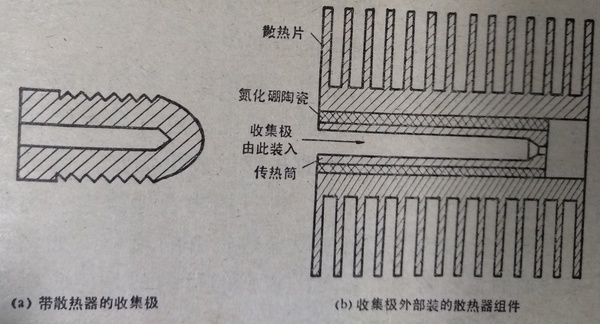
\includegraphics[width=0.75\linewidth]{figure/ch8-1}
	\caption{ 收集极散热装置示意图}
	\label{ch8-1}
\end{figure}

\subsection{带有翼片的散热器}


通常用铝制成,翼片的功能在于增加辐射面积。


为了增加散热器的辐射能力,通常是把散热器做成黑色的。
\subsection{散热块式散热器}

图\ref{ch8-2}所示是一种散热块式的散热器。这里收集极和散热块紧密地接触在一起。散热块一般用导热性能较好的紫铜或铝制成。它又和外包装体(即铝制外壳)紧密地接触在一起,整个外包装体用螺钉紧固在一块铝制的黑色散热平板上,散热平板再紧贴在整机上。这样,收集极的热量就先通过层层的传导,然后经对流及辐射散发到周围的空间中去。
\begin{figure}[phtb]
	\centering
	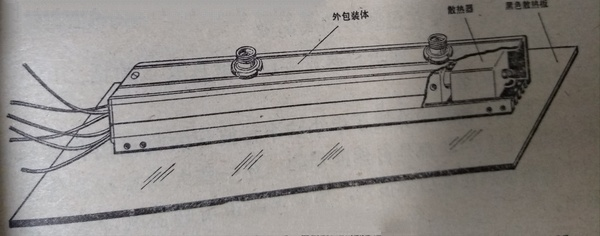
\includegraphics[width=0.75\linewidth]{figure/ch8-2}
	\caption{ 散热块式散热器}
	\label{ch8-2}
\end{figure}

在上面所讲的两种散热器中,必须使收集极和散热器接触得很紧密,为此,就需要提高机加工精度。也有采用锥面配合就是把收集极的外形和散热器的孔都做成锥面形,利用斜度使两者严密接触,如图\ref{ch8-3}所示。也有把两者焊接在一起的。还有的在收集极和散热器之间涂以导热良好的填料,如氮化硼粉和甲基硅油的混合物等。总之,它们的目的都是使收集极和散热器之间的热接触良好,以利于传导散热。
\begin{figure}[phtb]
	\centering
	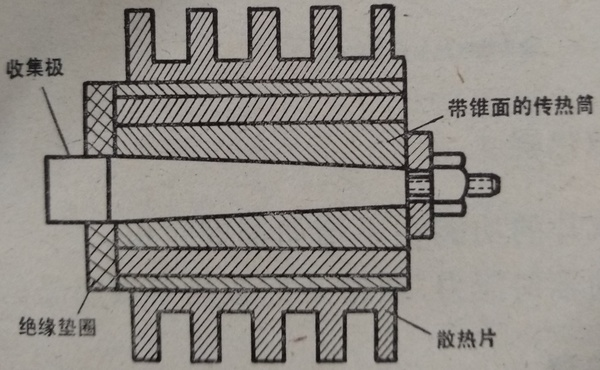
\includegraphics[width=0.55\linewidth]{figure/ch8-3}
	\caption{收集极和散热器之间锥面配合示意图}
	\label{ch8-3}
\end{figure}

还有一种行波管的散热结构,如图\ref{ch8-4}所示。这是在包装体的底部做出一条条的散热片。如果行波管工作时垂直放置的话,可以加强对流方式的散热。
\begin{figure}[phtb]
	\centering
	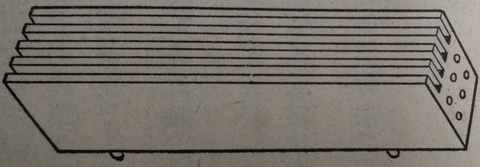
\includegraphics[width=0.55\linewidth]{figure/ch8-4}
	\caption{ 包装体上带有散热结构示意图}
	\label{ch8-4}
\end{figure}

上面我们简要地介绍了中小功率行波管的收集极和散热器的结构。它们一般都是自然冷却的。在一些大功率行波管中由于收集极热耗散功率很大,所以常常采用强迫风冷或液冷来散热。



对于大功率行波管收集极的结构,近年来已采用电子计算机来对收集极电子轨迹进行计算,以得到最佳的收集极形状。

最后,谈一谈散热块式的散热器和收集极之间的绝缘问题。这在螺旋线直接耦合的降压收集极行波管中是不可避免的(螺旋线直接耦合条件下,螺旋线必须接地以保证安全)。我们已经说过,为了减少收集极的热耗散,常常采用降压收集极的办法,这样,收集极的电压就要低于螺旋线电压。由于散热系统是裸露在外面的,为了保证安全,就要让它的电位和地电位一样,那么螺旋线电位就要高于地电位。但是对于某些输能方式(如直接耦合方式)来说,螺旋线又是必须接地的(同样是为了安全),这就发生了矛盾。解决这个矛盾的办法是在收集极和散热器之间夹上一层既绝缘又导热的物质。这样就允许收集极的电位比地电位低。同时,收集极的热量仍然可以通过和地同电位的散热器散发出去。人们经过试验找到了这样的材料,常见的有氧化铍陶瓷,氮化硼陶瓷和氧化铝陶瓷等。


图\ref{ch8-5}画出了收集极散热器的一种结构,中间的圆环就是用氮化硼或氧化铝陶瓷做成的。氧化铍陶瓷因为毒性大,不易加工,因此,在不十分必要时常被其它材料所代替。
\begin{figure}[phtb]
	\centering
	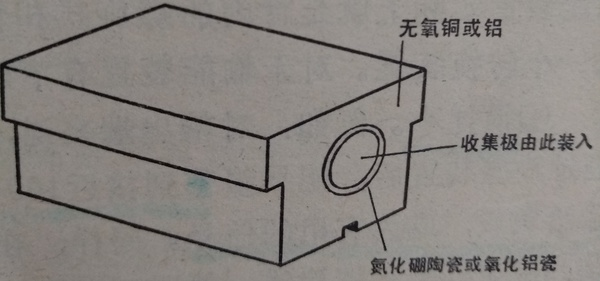
\includegraphics[width=0.55\linewidth]{figure/ch8-5}
	\caption{ 用于降压收集极的散热器示意图}
	\label{ch8-5}
\end{figure}



